\chapter{Representation of Music Information}

The representation of music, a multifaceted and intricate domain, plays a crucial role in the comprehension and analysis of musical works. Music, inherently abstract and temporal, can be encapsulated in two primary forms of representation: \emph{audio} and \emph{symbolic}.

Audio representation captures the live or recorded sound of music, preserving the performance's temporal and dynamic qualities. This form of representation is essential in fields such as musicology, audio engineering, and digital music processing, where the actual sound and its nuances are of prime interest. The shift from a symbolic to an audio-based representation marks a transition from a visual and interpretative medium to a direct auditory experience of music.

Symbolic music representation translates musical ideas into structured symbols. This encompasses the abstract musical qualities such as pitch, rhythm, and dynamics through established notational systems such as Western sheet music and digital formats like MIDI (Musical Instrument Digital Interface). Western sheet music, with its historical roots and standardized notation, provides a visual framework for interpreting and performing music. These notations, evolved over centuries, encompass various elements like notes on staves, clefs, key signatures, and time signatures, which collectively guide the performer in realizing the composer's intent. While the internal structure of a music score is not a focus of this work, a curious reader may find useful information in \cite{Read1969}.

Different music representations offer distinct insights and tools for understanding, analyzing, and transforming music. This chapter delves into these two primary ways of representing music, defining basic notions around these.

\section{Audio Signals}

Audio-based music representation refers to a form of signal representation. The most prevalent of these is the \emph{waveform}, a real-valued function in the time domain that represents the temporal amplitude of a sound. Another common signal representation is the \emph{spectrogram}, which provides information about the local\footnote{With respect to the time domain.} frequency distribution within an audio sample.

Although this form of representation is not the primary focus of this work, understanding certain notions is beneficial for a more comprehensive grasp of the general \emph{Automatic Music Transcription} framework, of which \emph{Performance MIDI to Score Transcription} is a part.

\subsection{Waveform}

In the digital world, the audio is not a continuous signal but discrete one. The transformation from a continuous-time signal to a discrete-time signal is called \emph{sampling}. During this process, a single value of the signal at a specific point in time is referred to as a \emph{sample} \cite[p.~34--35]{Smith1999}. Additionally, an entire sample recording is sometimes called an \emph{audio sample}.

\begin{figure}[ht!]
\centering
\includesvg[width=\textwidth]{images/sampling_rate.svg}
\caption[An example of a sampling a sine wave with different sampling rates.]{An example of a sampling a sine wave of the frequency $500$ Hz with different sampling rates: $f_s = 8\,000$ Hz and $f_s = 32\,000$ Hz. The quality of the audio is degraded but the sampling fidelity is better for the higher sampling rate.}
\end{figure}

There are two main parameters of sampling process which directly affect the overall quality of the obtained sound:
\begin{itemize}
   \item \emph{Sampling rate} --- the average number of samples in one second.
   \item \emph{Bit depth} --- the number of bits that one sample encodes.
\end{itemize}

\begin{figure}[ht!]
\centering
\includesvg[width=\textwidth]{images/bit_depth.svg}
\caption[An illustration of bit depth affecting the quality of an audio.]{An illustration of bit depth affecting the quality of an audio: a sine wave of the frequency $500$ Hz sampled with two different vertical resolutions: $2$-bit and $4$-bit. The $2$-bit sample barely reflects the original signal. Sampling rate is assumed to be infinite.}
\end{figure}

The sampling rate sets an upper limit on the frequency that can be accurately represented in a discrete signal. This principle is conveyed by the \emph{Nyquist–Shannon sampling theorem} \cite[p.~40]{Smith1999}. On the other hand, the bit depth refers to the vertical resolution of a sound, determining the dynamic range of the signal \cite[p.~36]{Smith1999}.

Waveform representation easily allows the analysis of amplitude peaks and the audio envelope, which includes aspects of audio dynamics: attack, sustain, decay, and release of a sound.

\subsection{Spectrogram}

The waveform representation is not the only one possible way of encoding an audio signal. Each signal can be decomposed into frequencies, meaning that each (regular enough) function can be viewed as a sum of trigonometric functions. More precisely, a regular enough (i.e. continuous) real-valued function $f\colon\left[-\tfrac{P}{2},\tfrac{P}{2}\right]\to\mathbb{R}$ can be expressed as an infinite series: \[f(x) = \sum_{n=-\infty}^{+\infty}c_n e^{2\pi i\frac{n}{P}x}\] where $c_n$ is defined as: \[c_n = \frac{1}{P}\int\limits_{-\tfrac{P}{2}}^{\tfrac{P}{2}}f(x)e^{-2\pi i \frac{n}{P}x}\mbox{d}x\] for $n\in\mathbb{Z}$. See \cite[p.~185--186]{Rudin1976} for more details.

When a Fourier transform is applied to short time windows of a discrete signal using \emph{Discrete Short-time Fourier Transform} (DSTFT), a series of signal frequency decompositions is obtained. The process results in a \emph{spectrogram}, a visual representation of an audio signal. A spectrogram displays how the intensity of various frequency components changes over time, offering a detailed view of the signal's frequency spectrum \cite[p.~365--366]{Smith1999}.

\begin{figure}[ht!]
\centering
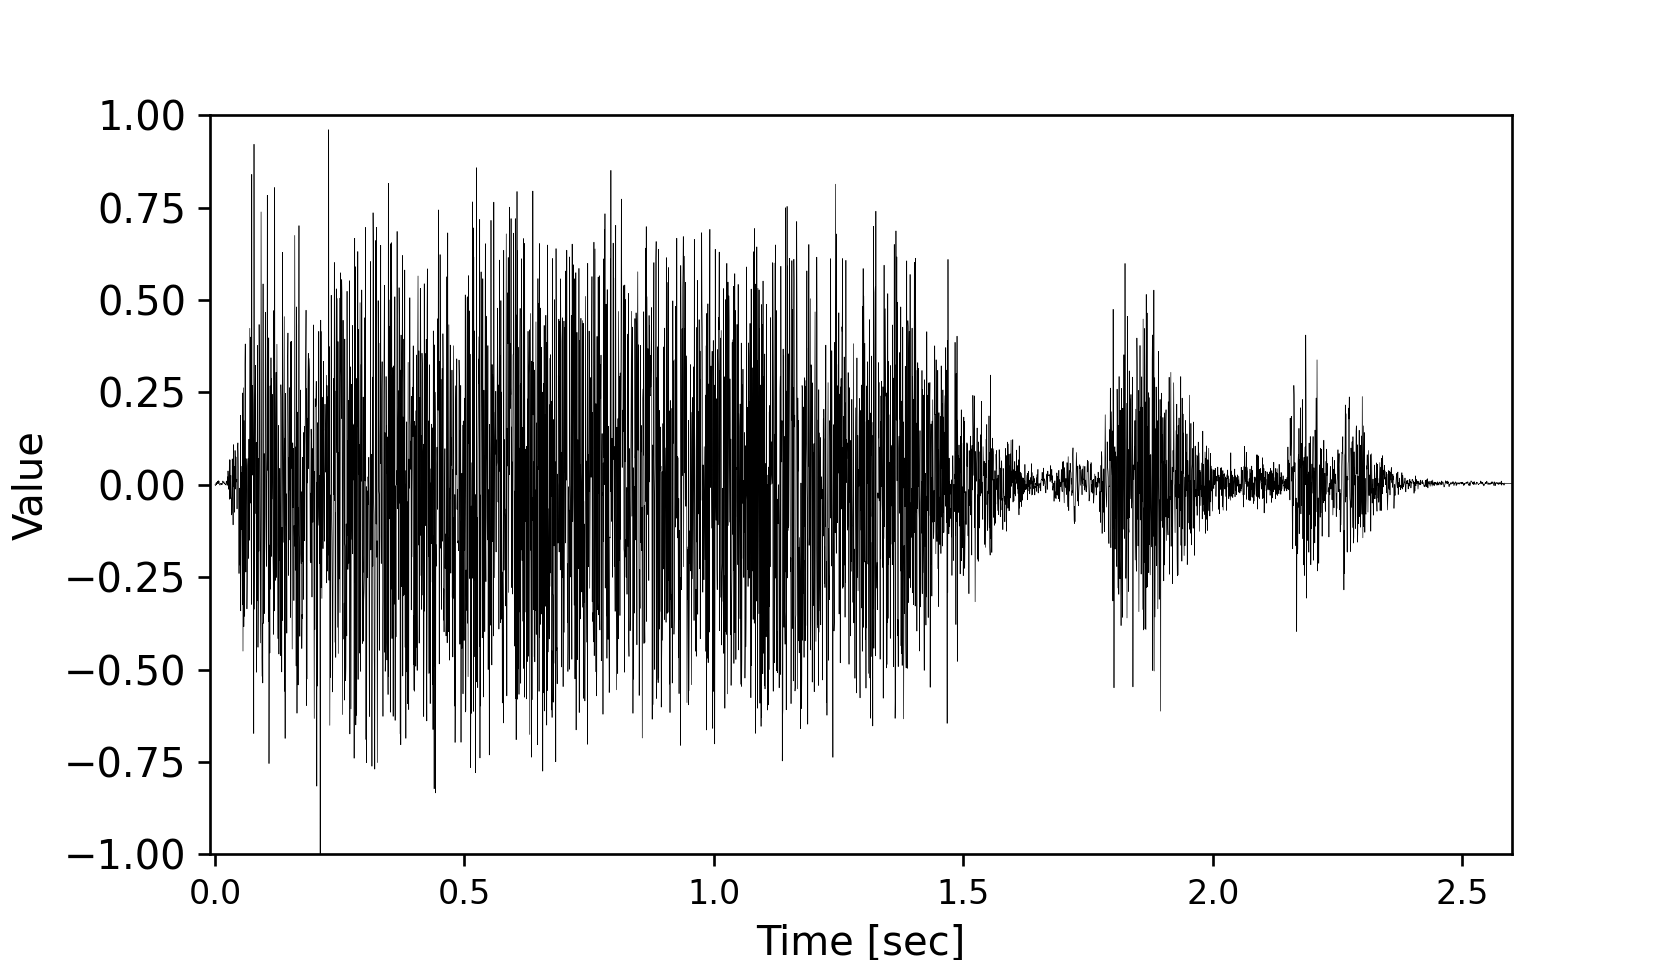
\includegraphics[width=0.49\textwidth]{images/waveform.png}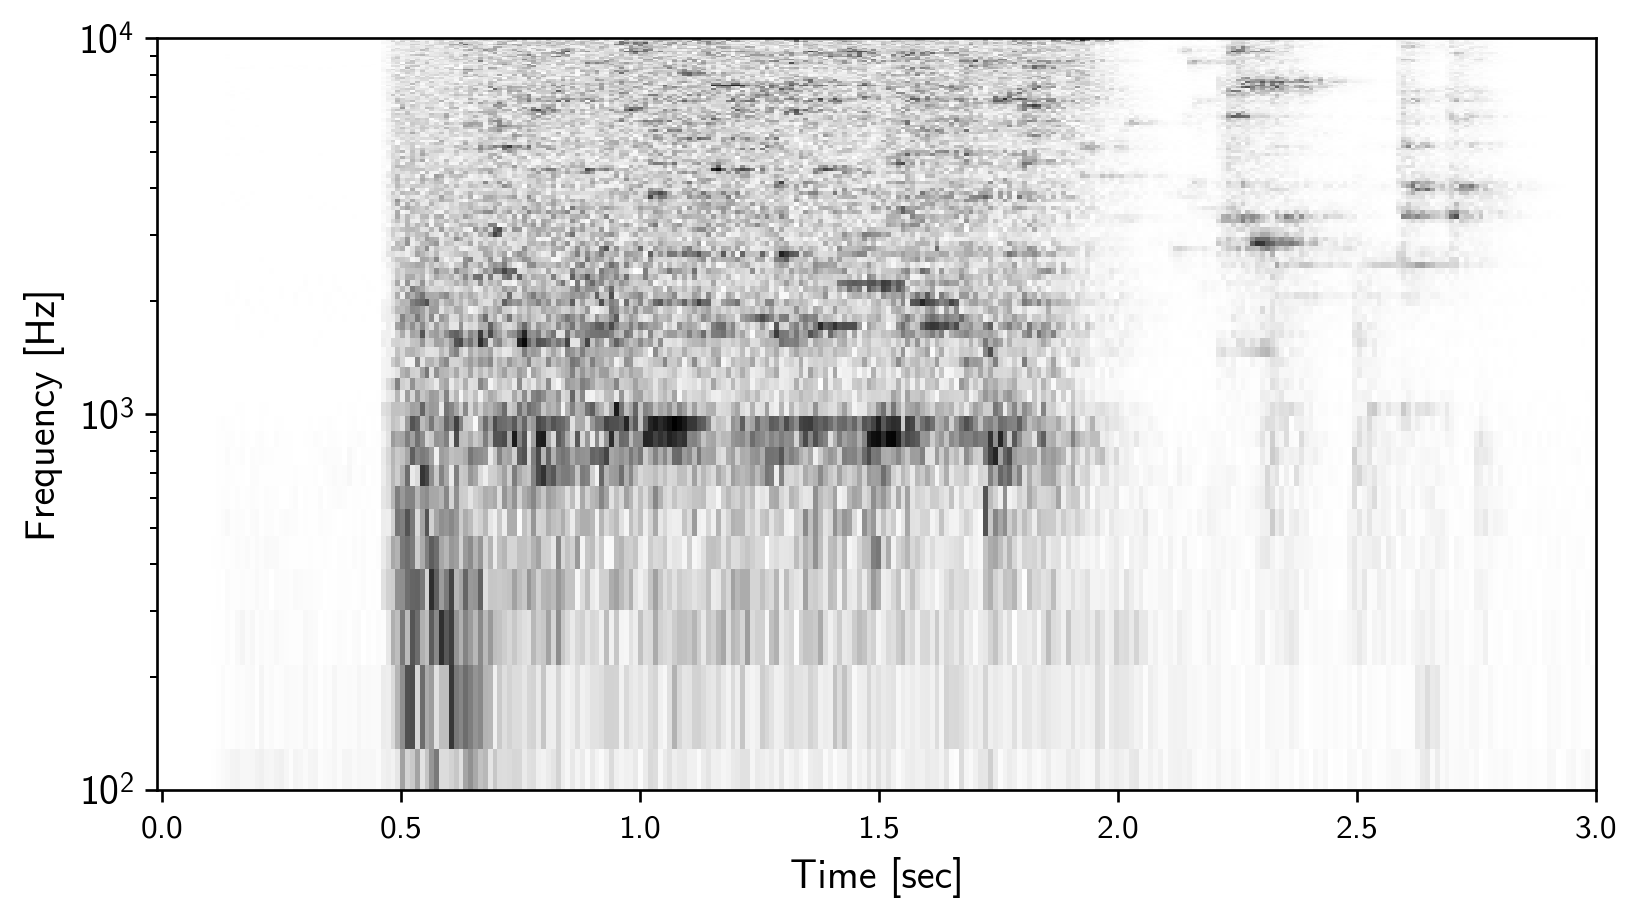
\includegraphics[width=0.49\textwidth]{images/spectrogram.png}
\caption[A comparison of two different representations of the same sound.]{A comparison of two different representations of the same sound: a glass break: \emph{waveform} (left) and \emph{spectrogram} (right). The audio is rich in various frequency bands.}
\end{figure}

The spectrogram representation is vital for frequency information retrieving frequency information, aiding in the extraction of features such as pitch (the fundamental frequency) and timbre. However, short-time Fourier transforms are constrained by a trade-off between time and frequency resolutions. Achieving high resolution in one inherently limits the resolution in the other \cite[p.~365--366]{Smith1999}.

\section{Symbolic Representation}

Symbolic representation encodes music through structured, discrete set of symbols, which abstracts certain musical elements such as pitch, duration or dynamics. The ISO/IEC 14496-23:2008 defines \emph{Symbolic Music Representation} (SMR) as \emph{a logical structure based on: symbolic elements representing audiovisual events, the relationship between those events, and aspects related to how those events can be rendered (visually as music notation or audibly) and synchronized with other media types} \cite{ISO2008}.

The definition encompasses various forms of a musical notation, with traditional sheet music as the most established form.

\subsection{Sheet Music}

\emph{Sheet music}, also known as a \emph{score}, is a form of musical notation that can be handwritten or printed. It utilizes musical symbols to represent various elements such as the pitches, rhythms, and chords of a song or an instrumental piece \cite{Wiki2024B}. Sheet music provides essential information that enables musicians to perform a piece.

There are many forms of sheet music notation, originated in different cultures. The music notation of our interest is the notation of Western Classical Music, originated in Europe.

\begin{figure}[ht!]
\centering
\includesvg[width=\textwidth]{images/prelude_gen.svg}
\caption[First bars of Frédéric Chopin's \emph{Prelude Opus 28, No. 4}.]{First bars of Frédéric Chopin's \emph{Prelude Opus 28, No. 4} \cite{Chopin1839}.}
\label{prelude_opus_28_4}
\end{figure}

Western sheet music is a symbolic representation of music that employs a set of standard notations to convey the elements of a musical composition. Key elements include:
\begin{itemize}
   \item \emph{Staff}: Consisting of five horizontal lines and four spaces, each representing a different musical pitch \cite[p.~27]{Read1969}.
   \item \emph{Clef}: Positioned at the beginning of the staff, it specifies the pitch of the notes on the staff (e.g., treble clef $\clefGInline$, bass clef $\clefFInline$ \cite[p.~51--55]{Read1969}. For instruments of a wide pitch range (such as piano), it may change during the course of a piece to accommodate the varying pitch ranges.
   \item \emph{Notes and Rests}: Symbols that represent the pitch and duration of musical sounds and silences, such as whole note $\wholeNote$, half note $\halfNote$, quarter note $\quarterNote$, etc., and corresponding rests like whole rest $\wholeNoteRest$, half rest $\halfNoteRest$, quarter rest $\crotchetRest$, etc. Dotted notes, like the dotted half note $\halfNoteDotted$, are extended by half their length, equating to three quarter notes in this example. For further information, refer to \cite[p.~64--65, 96, 103, 113--114]{Read1969}.
   \item \emph{Key Signature}: Indicates the music's key by specifying consistently altered \emph{flats} ($\flat$) or \emph{sharps} ($\sharp$) \cite[p.~135--136]{Read1969}. For example, a sharp symbol $\sharp$ next to the clef: \[\includesvg{images/key_signature_gen.svg}\] as seen in Figure \ref{prelude_opus_28_4}, signifies that each note on the indicated line should be played a semitone higher (in this case, $\textrm{F}\sharp$ instead of $\textrm{F}$), corresponding to the $\textrm{E}$ minor scale (enharmonically equivalent\footnote{Two notes are \emph{enharmonically equivalent} if they have the same pitch but are notated differently \cite[p.~10]{Kostka1994}. This is a property of the standard twelve-tone equal temperament tuning (12-ET). Other tuning systems may not have this property.} to $\textrm{G}$ major).
   \item \emph{Tempo Marking}: Indicates a song's tempo, specifying the duration of a note. This can be an exact beats per minute (BPM) value, such as $\quarterNote =90$, or described conventionally using Italian terms, ranging from \emph{larghissimo} (extremely slow, under 40 BPM) to \emph{prestissimo} (extremely fast, over 208 BPM) \cite[p.~276--277]{Read1969}.
   \item \emph{Time Signature}: Dictates the rhythmic structure by defining the number of beats per measure and the note value for one beat \cite[p.~148--150]{Read1969}. Represented as a fraction $\mathbf{\genfrac{}{}{0pt}{2}{n}{m}}$, with the denominator $m$ being a power of 2. For example, $\lilyTimeSignature{3}{4}$ indicates three quarter notes per measure. Common time signatures like $\lilyTimeC$ and $\lilyTimeCHalf$ are equivalent to $\lilyTimeSignature{4}{4}$ and $\lilyTimeSignature{2}{2}$, respectively.
   \item \emph{Dynamics}: Symbols and terms indicating the volume of the music, marked from $\lilyDynamics{ppp}$ (pianississimo), through $\lilyDynamics{mp}$ (mezzo piano) and $\lilyDynamics{mf}$ (mezzo forte), to $\lilyDynamics{fff}$ (fortississimo) \cite[p.~250]{Read1969}. These markings are interpretative and not absolute.
   \item \emph{Articulation Marks}: Instructions on the execution of notes, such as staccato or legato, visually represented by accents and slurs \cite[p.~260--268]{Read1969}.
\end{itemize}

A score of a music piece is comprehensive enough to encapsulate a variety of musical elements, serving as a detailed blueprint for performers to interpret and bring to life the composer's intentions. However, the sheet notation as it is cannot be used by computers directly. Thus we need to limit ourselves only to digital representations of musical scores.

\subsection{Musical Instrument Digital Interface}

The standard for music communication is \emph{Musical Instrument Digital Interface} (MIDI). However the term MIDI is overloaded and means usually several things:
\begin{itemize}
   \item A protocol enabling musical information (notes, velocities, control signals) communication between electronic devices.
   \item A technical standard detailing the specifications for digital interfaces and hardware connectors.
   \item An abstraction representing musical information encompassed within the MIDI protocol.
   \item A file format that stores a sequence of recorded MIDI messages.
   \item A MIDI stream, or a content of a MIDI file.
\end{itemize}

The specific interpretation of MIDI depends on the context. In this work, \emph{performance MIDI} refers to the last point, where the stream is captured through a digital piano or other MIDI-compatible digital keyboards\footnote{Although MIDI is not exclusively used for keyboards, the primary focus of the deep learning methods discussed here is on piano compositions.}.

A MIDI stream comprises events, each consisting of two components: a MIDI time and a MIDI message. The time value indicates the duration to wait before executing the next message in the MIDI data sequence \cite[p.~3]{Oliveira2017}. There are two principal message types:
\begin{itemize}
\item \emph{Note on}: Sent when a performer presses a key on an instrument.
\item \emph{Note off}: Triggered when a player releases a key, turning off the corresponding note.
\end{itemize}

Each message specifies two values: \emph{pitch} and \emph{velocity}\footnote{A note intensity, usually correlated with the volume, but not necessarily. This term derives from how some digital instruments measure the speed at which a key is pressed. Some instruments may not respond to this attribute at all \cite[p.~22]{Huber2007}.}. All values are encoded by a $7$-bit integer, from $0$ to $127$.

MIDI streams do not encode sound nor they specify it. The sound rendering is not a responsibility of the MIDI protocol.

The MIDI standard is built upon the 12-tone equal temperament (12-ET) system, which divides an octave into 12 logarithmically equal parts\footnote{The frequency of a note is perceived logarithmically.}. This system is represented in the conventional 88-key keyboard layout, ranging from $\textrm{A}0$ to $\textrm{C}8$, corresponding to MIDI pitch values within the range of $[21, 108]$. The relationship between frequency and pitch in standard tuning\footnote{The widely accepted standard tuning, A440, established by ISO \cite{ISO1975}, sets the frequency of the $\textrm{A}4$ note at $440$ Hz. This $\textrm{A}4$ note corresponds to the MIDI pitch value of $69$.} is expressed by the formula: \[m = 12 \log_2\left(\frac{f_m}{440\textrm{ Hz}}\right) + 69\] where $m$ is the pitch for a given frequency $f_m$ \cite[p.~47--48]{MIDI1996}.

\begin{figure}[ht!]
\centering
\resizebox{1.0\linewidth}{!}{
\begin{tikzpicture}

\coordinate (origin) at (0,0);
\coordinate (stave) at (origin);
% left line of first key
\draw (9.25,-1) -- (9.25,-5);

\def\midiC{0}
\def\midiD{2}
\def\midiE{4}
\def\midiF{5}
\def\midiG{7}
\def\midiA{9}
\def\midiB{11}

% Define a command to calculate the MIDI note number
\newcommand{\midiNote}[3]{% #1 is pitch, #2 is octave
    % Assign MIDI note numbers to each pitch (C=0, C#=1, D=2, ..., B=11)
    \pgfmathtruncatemacro{\pitchValue}{\csname midi#1\endcsname}
    \pgfmathtruncatemacro{\midiNumber}{12 + \pitchValue + #2 * 12 + #3}
};

\newcommand{\drawPianoKey}[4]{
	\pgfmathparse{#2*7+\p+0.25-#3}
        \edef\myx{\pgfmathresult}
        % draw three lines for top, right, bottom of this key
        \draw (\myx,-1) -- (\myx,-5);
        \draw (\myx,-1) -- ($(\myx,-1)+(-1,0)$);
        \draw (\myx,-5) -- ($(\myx,-5)+(-1,0)$);
        % print pitch on line
        \node [anchor=base,xshift=-15] at (\pgfmathresult,-4.5) {{#1}{#2}};
        
		\midiNote{#1}{#2}{0};
    		\node[anchor=base,xshift=-15] at (\pgfmathresult, -5.5) {\midiNumber};

        \blacknotefalse
        \ifcase\p
        \or
            \blacknotetrue
        \or
          \ifnum#2>0
            \blacknotetrue
          \fi
        \or
        \or
            \blacknotetrue
        \or
            \blacknotetrue
        \or
            \blacknotetrue
        \else
        \fi
        \ifblacknote
            % recalculate x
            \pgfmathparse{#2*7+\p-#3}
                \fill ([xshift=0.25cm, yshift=-1cm]stave.south -| \pgfmathresult,0) ++(-0.25cm,0) rectangle ++(0.5cm,-2.5cm);
                % print pitch on black key
                \node [anchor=base,xshift=0.25cm,white] at (\pgfmathresult,-2.5) {\textbf{#1}$\sharp$};
		        \midiNote{#1}{#2}{1};
    		       \node[anchor=base,xshift=0.25cm] at (\pgfmathresult, -0.75) {\midiNumber};
        \fi
}

\newif\ifblacknote
\foreach \octave in {2,...,5}
    \foreach \pitch [count=\p] in {C,D,E,F,G,A,B}{
        % calculate x position from octave and pitch
        \drawPianoKey{\pitch}{\octave}{5}{15}
    }

\def\p{7}
\drawPianoKey{C}{6}{11}{21}
\end{tikzpicture} 

}
\caption[A piano keyboard layout with 49 keys.]{A piano keyboard layout with 49 keys. The integers stand for MIDI note values.}
\end{figure}

A velocity value for a played note should be non-zero, typically controlling the volume of the note. However, there is no universal agreement on the exact gain corresponding to a given velocity value.

The smallest MIDI time unit is \emph{tick}. The length of a single tick is determined by two MIDI parameters:
\begin{enumerate}
	\item \emph{tempo}, which describes microseconds per quarter note.
	\item \emph{ticks-per-quarter-note}, with a common value of $480$.
\end{enumerate}

For example, in the tempo of 120 beats per minute (BPM) the quarter note lasts 500,000 microseconds. In that case, assuming 480 ticks per quarter note, one tick lasts: \[\textrm{tick length} = \frac{\text{ 500,000 microseconds}}{\text{480 ticks}} = 1041.67 \text{ microseconds}\] This feature allows MIDI to handle both physical lengths, as well as musical ones.

While this work primarily focuses on MIDI representation, other notable symbolic representations include:
\begin{itemize}
   \item \emph{MusicXML}: An XML-based file format for representing Western musical notation, designed for both human and machine readability \cite{Good2001}.
   \item \emph{ABC}: A simplified musical notation system encoding essential musical elements \cite{ABC2013}.
   \item \emph{LilyPond}: As authors claim, \emph{LilyPond} is \emph{designed to solve the problems we found in existing software and to create beautiful music that mimics the finest hand-engraved scores} \cite{LilyPond2002}. \emph{LilyPond} has been used to generate all scores and musical glyphs present in this dissertation.
\end{itemize}

Symbolic notation has its limitations: it can only describe predefined musical aspects, ignoring a multitude of other factors\footnote{This is, as any kind of abstraction, rather a desired property.}. For instance, the sheet notation does not capture the timbre of sound and is very limited in expressing dynamic sound ranges. While the format was not primarily designed to represent symbolic music but to allow communication between musical devices, it may be used for that purpose as it can handle 	musical as well as physical onset times and note durations\cite{Grohganz2014}.

Most symbolic representations are based on the standard division of an octave into 12 tones, which makes them less suitable for music from non-Western European traditions, such as the Indonesian pentatonic \emph{slendro} or seven-note \emph{pelog} systems, for gamelan instruments \cite[p.~73]{Sethares2005}. Certain music genres, like \emph{musique concrète}, are not expressible through traditional notation at all \cite[p.~69--77]{Schaeffer2012}.

In the context of this work, we limit ourselves to the heritage of Western European Music, as we are focused on classical European piano works, composed by Bach, Mozart, Beethoven, Schubert, Chopin, Liszt and others.
